\chapter{Concept Mapping}


\begin{figure}[ht]
    \centering
    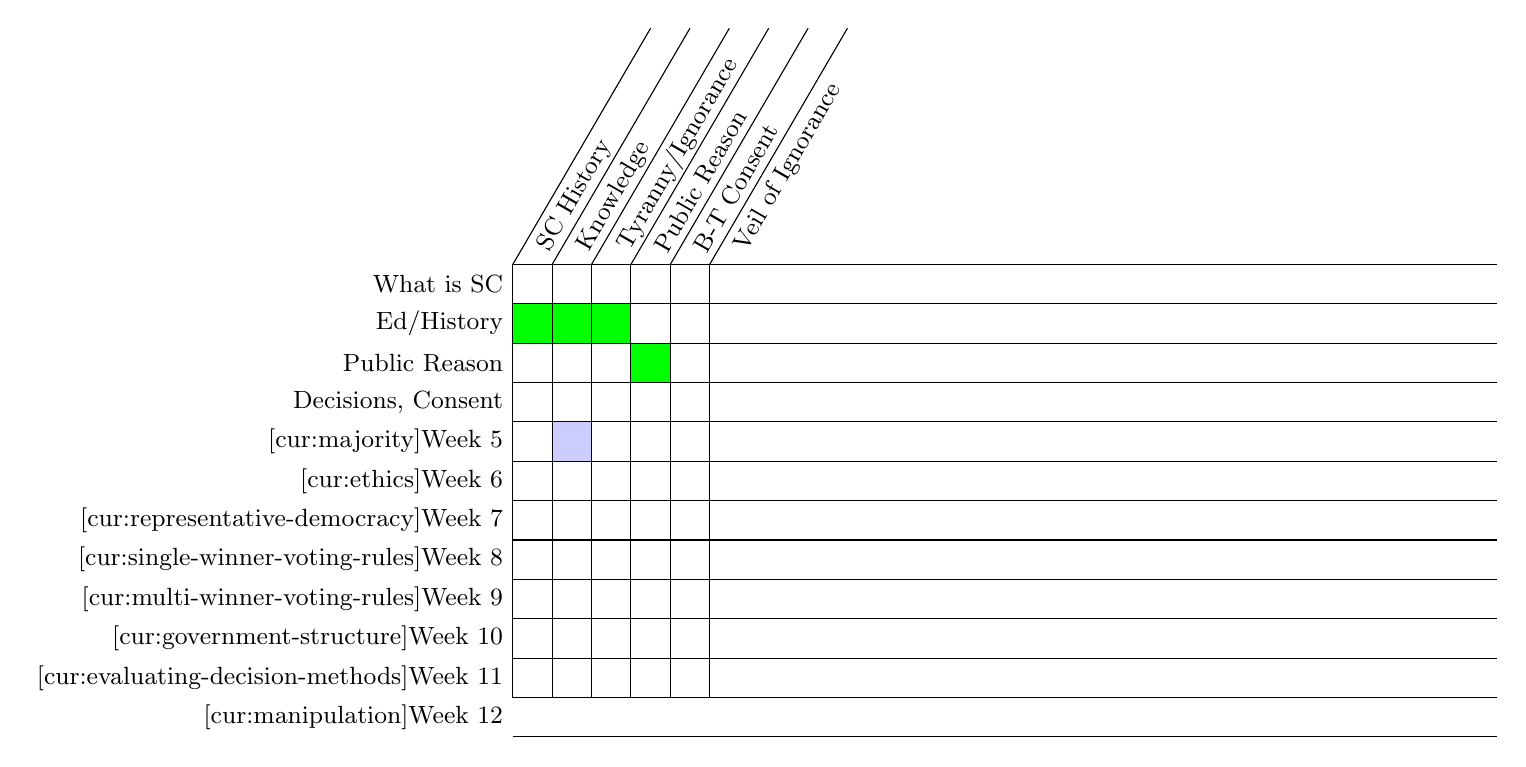
\begin{tikzpicture}[
        %sibling distance=10em,
        font=\small,
        ]
    \foreach \x[count=\xi from 0] in {
        2,2,2,
        3}
    {
        \draw [fill=green] (\xi/2,0.5-\x/2) rectangle ++(0.5,-0.5);
    }
    \foreach \x / \y in {
        1/6}
    {
        \draw [fill=blue!20] (\x/2,1-\y/2) rectangle ++(0.5,-0.5);
    }
    \foreach \x[count=\xi] in {
        SC History,
        Knowledge,
        Tyranny/Ignorance,
        Public Reason,
        B-T Consent,
        Veil of Ignorance}
    {
        \node at (0.5*\xi-0.35,0) [anchor=south west] {\rotatebox{60}{\x}};
        \draw (0.5*\xi-0.5,0) -- ++(1.75,3);
        \draw (0.5*\xi-0.5,0) -- ++(0,-12/2+0.5);
    }

    \draw (0,0) -- (12.5,0);
    \foreach \x[count=\xi] in {
        What is SC,
        Ed/History,
        Public Reason,
        {Decisions, Consent},
        \hyperref[cur:majority]{Week 5},
        \hyperref[cur:ethics]{Week 6},
        \hyperref[cur:representative-democracy]{Week 7},
        \hyperref[cur:single-winner-voting-rules]{Week 8},
        \hyperref[cur:multi-winner-voting-rules]{Week 9},
        \hyperref[cur:government-structure]{Week 10},
        \hyperref[cur:evaluating-decision-methods]{Week 11},
        \hyperref[cur:manipulation]{Week 12}
    }
    {
        \node at (0,-0.5*\xi+0.25) [anchor=east] {\x};
        \draw (0,-0.5*\xi) -- (12.5,-0.5*\xi);
    }

    \end{tikzpicture}
    \caption{\label{fig:concept-map}Concept mapping.}
\end{figure}